\documentclass{beamer}
% \usefonttheme{professionalfonts}
\usefonttheme{professionalfonts}

\usepackage{amsmath}
\usepackage{cancel}
%%%%%%%%%%%%%%%%%%%%%%%%% For making hand-outs %%%%%%%%%%%%%%%%%%%%%%%%%%%
% \documentclass[handout]{beamer}
% \usepackage{pgfpages}
% \pgfpagesuselayout{2 on 1}[a4paper,border shrink=5mm]
%%%%%%%%%%%%%%%%%%%%%%%%%%%%%%%%%%%%%%%%%%%%%%%%%%%%%%%%%%%%%%%%%%%%%%%%%%
\definecolor{inputred}{HTML}{c30e0e}
\definecolor{hiddenblue}{HTML}{2626c9}
\definecolor{outputgreen}{HTML}{008000}
\newcommand{\figheight}{0.72\textheight}
% \usepackage{eulervm}
\usepackage{default}
\usepackage{caption}
\usepackage{booktabs,mathptmx,siunitx}
% \usefonttheme{serif}
\graphicspath{{img/}}
\captionsetup{font=scriptsize, labelfont=scriptsize}


\usepackage{showexpl}



\begin{document}



\begin{frame}[fragile]

\centering\Huge Block Practical: Connectionist models and cognitive processes
\vfill \huge
\centering Part 4: \textbf{Replicating a Model} \large
\vfill
\textit{
Olivia Guest }

\end{frame}


\begin{frame}[fragile]
\frametitle{Why replicate?}
\framesubtitle{Not boring, repetitive?}
        \  \\

\begin{itemize}
\item<2-> A pillar of science: if studies do not replicate, then what?

\ \\

\ \\

 \item <3->Pedagogical: learn from ``better''/published research!
 
\ \\

 \ \\
 
\item<4-> Augment:  make model explain, predict more!

 
\ \\

 \ \\
 
\item<5-> Why start from scratch?
\end{itemize}


\end{frame}

\begin{frame}[fragile]
\frametitle{How to replicate?}
\framesubtitle{Not painful, tedious?}
        \  \\

\begin{itemize}
\item<2-> By being patient: you will end up being an expert in methodology, theory

\ \\

\ \\

 \item <3-> By reading up: papers usually provide neither equations nor code
 
\ \\

 \ \\
 
\item<4->  By being patient: programming takes time, running code takes time, etc.

 
\ \\

 \ \\
 
\item<5-> If you get stuck you can always ask the original authors!
\end{itemize}


\end{frame}

\begin{frame}[fragile]
\frametitle{Replication: The bigger picture}
\framesubtitle{We're doing cognitive science as well as coding!}
        \  \\

\begin{itemize}
\item<2-> What theory is this model part of?

\ \\

\ \\

 \item <3-> What assumptions is the model making, what assumptions is the theory making?
 
\ \\

 \ \\
 
\item<4-> Are implementation details important to the model, to the theory? 

 
\ \\

 \ \\
 
\item<5-> Does the model uniquely support a specific theory? 
\end{itemize}


\end{frame}
\begin{frame}[fragile]
\frametitle{Replication: The bigger picture}
\framesubtitle{We're doing cognitive science as well as coding!}
        \  \\

\begin{itemize}
\item<2-> What mechanism(s) is the model proposing?

\ \\

\ \\

 \item <3-> What are the model's predictions? 
 
\ \\

 \ \\
 
\item<4-> Can the model account for data it has not seen?

 
\ \\

 \ \\
 
\item<5-> How well does the model compare to other accounts?
\end{itemize}


\end{frame}

\begin{frame}[fragile]
\frametitle{Tyler et al. (2000)}
\framesubtitle{Conceptual Structure and the Structure of Concepts: A
Distributed Account of Category-Specific Deficits}
             \  \\

\begin{itemize}
\item<2-> Model for semantic memory after neurodegenation 

\ \\

\ \\

 \item <3-> Patients have category-specific deficit: animals $<$ artifacts

 \ \\
 
 \ \\
 
\item<4->features of living vs non-living things differ $\rightarrow$

their representations differ $\rightarrow$

their preservation after neurodegenation differs
\end{itemize}
\end{frame}

\begin{frame}[fragile]
\frametitle{Tyler et al. (2000)}
\framesubtitle{Example of patient's ability to draw common items}

\begin{figure}[t]
 \begin{flushleft}
\centering
 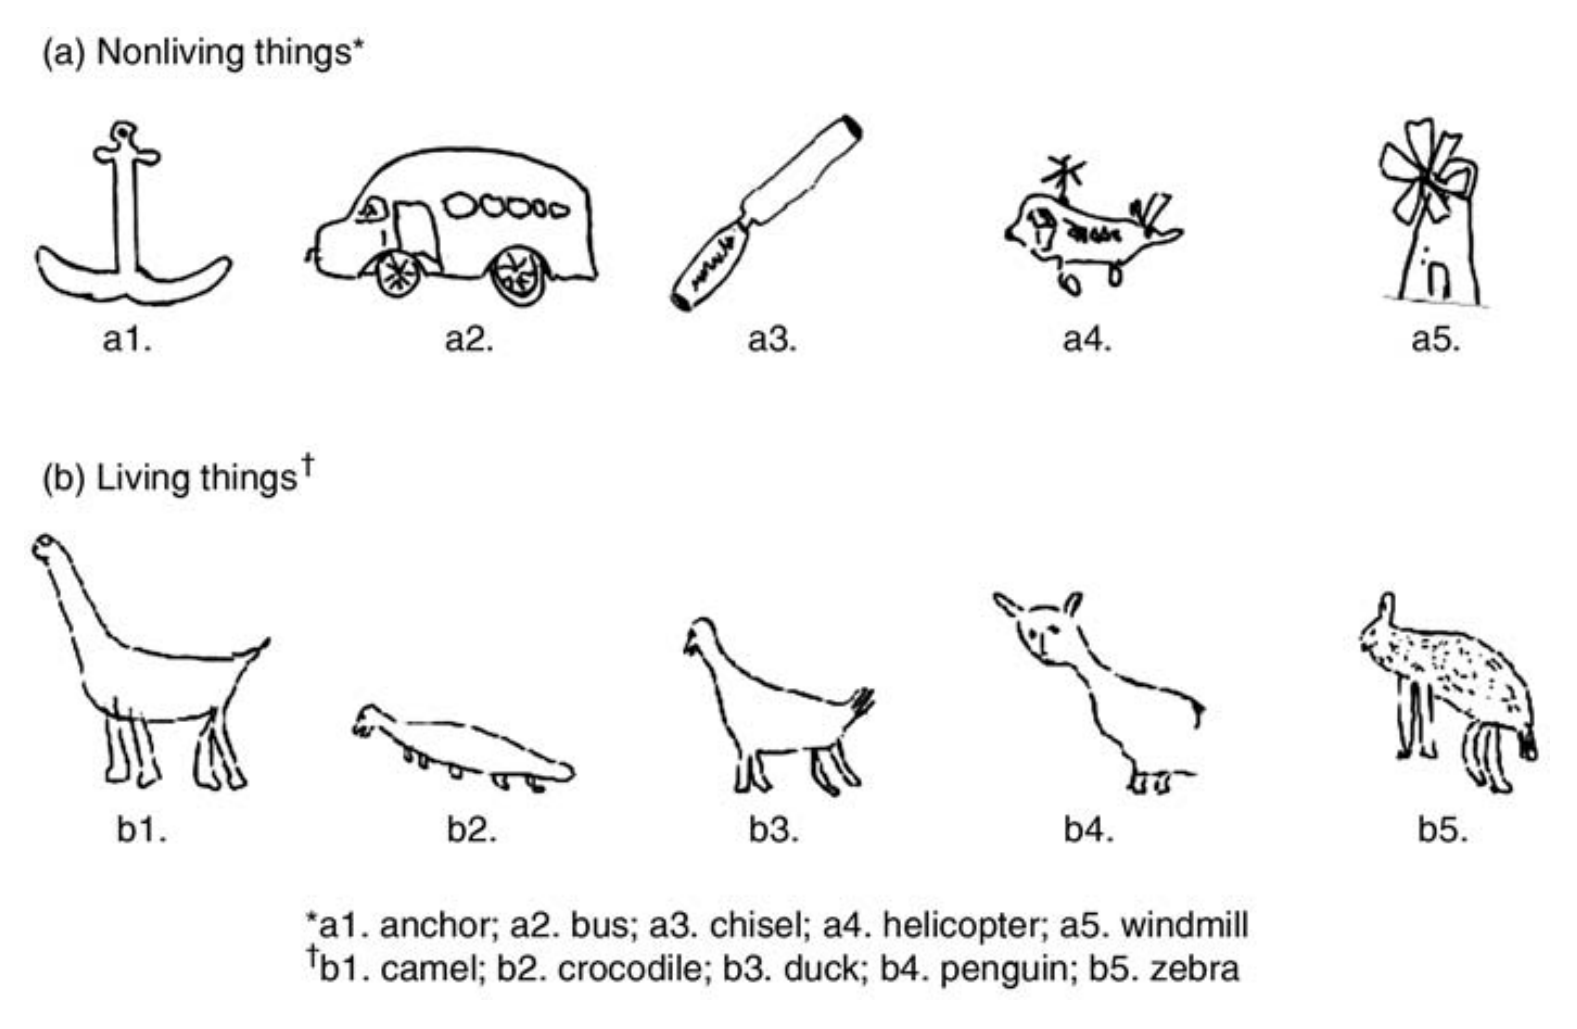
\includegraphics[scale=.26]{./fig/taylor_2000.png}


 \end{flushleft}

 \end{figure}
\end{frame}

\begin{frame}[fragile]
\frametitle{Tyler et al. (2000)}
\framesubtitle{To replicate we need...}
 \begin{columns}[T]
    \begin{column}{.45\textwidth} 
             \  \\
 \   \\   
     
     
\begin{itemize}[<+->]
\item The architecture: connectivity, widths of each layer, etc.

\ \\

 
\item The learning algorithm: epoch size, momentum, learning rate, etc.

\ \\

 
 \item The environment: input and target patterns!
\end{itemize}
\end{column}
\begin{column}{.55\textwidth}
\begin{figure}[t]
 \begin{flushleft}

 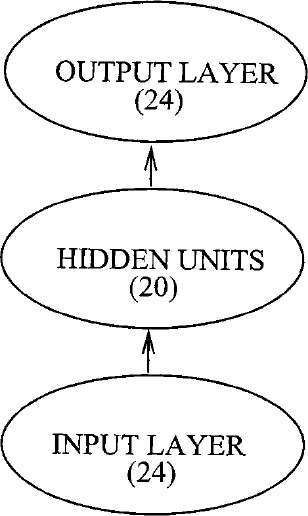
\includegraphics[height = \figheight]{./fig/tyler00.png}


 \end{flushleft}
\end{figure}
\end{column}

\end{columns}
\end{frame}


\end{document}
